\documentclass{beamer}
\usepackage{pgffor,pgfmath}
\usepackage{lipsum}
\usepackage{multicol}
\usetheme{ucla}
\usepackage{graphicx}
\usepackage{listings}
\usepackage{verbatim}
\usepackage{tikz}
\linespread{1.5}
\usepackage{comment}

\usepackage{amsmath, amsthm, amssymb, latexsym}

%\newtheorem{definition}{Definition}

\title{Lecture 2}
\author{Charles Rambo}
\institute{UCLA Anderson School of Management}
\date{2023}
\location{Los Angeles, California}

% Turn on slide numbers:
\showSlideNumber{}

\AtBeginSection[]
{
    \begin{frame}
        \frametitle{Table of Contents}
        \tableofcontents[currentsection]
    \end{frame}
}


\begin{document}

\insertTitleSlide


\begin{frame}
\frametitle{Table of Contents}
\tableofcontents
\end{frame}

\section{Integration}

\subsection{Riemann Integration}

\begin{frame}
\frametitle{Definite Integration}
\begin{center}
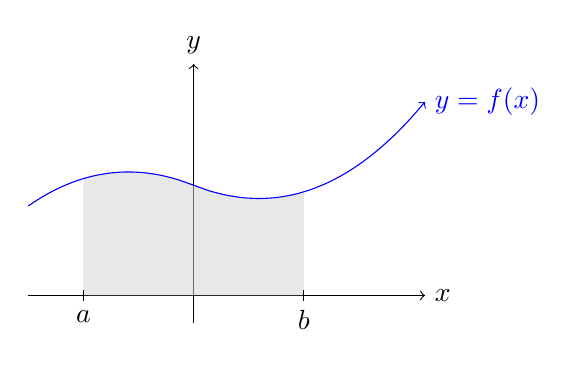
\begin{tikzpicture}[declare function = {f(\x) = 0.005 * \x^3 + 0.16 * \x^2 - 0.4 * \x + 2;}, scale = 0.7]
  \draw[->] (-3, 0) -- (4.2, 0) node[right] {$x$};
  \draw[->] (0, -0.5) -- (0, 4.2) node[above] {$y$};
  \fill [gray!35, domain=-2:2, variable=\x, opacity = 0.5]
  (-2, 0) -- plot ({\x}, {f(\x)}) -- (2, 0) -- cycle;
  
  \draw[->, domain=-3:4.2, smooth, variable= \x, blue] plot ({\x}, {f(\x)}) node[right] {$y = f(x)$};
  
  \draw (-2, 0.1) -- (-2, -0.1) node[below] {$a$};
  \draw (2, 0.1) -- (2, -0.1) node[below] {$b$};  
\end{tikzpicture}
\end{center}
The motivating problem for the definite integral is finding area under the graph $y = f(x)$ for $a \leq x \leq b$.
\end{frame}

\begin{frame}
\frametitle{Riemann Sum}
\begin{Definition}
Suppose we have a function $f$ defined on the interval $[a, b]$. Consider a {\bf partition pair} $P$ and $T$; $P = (x_0, x_1, \ldots x_n)$ and $T = (t_1, t_2, \ldots, t_n)$, where
$$
a = x_0 \leq t_1 \leq x_1 \leq \ldots\leq x_{n-1} \leq t_n \leq x_n = b.
$$ 
The {\bf Riemann sum} corresponding to the partition pair $P$ and $T$ is defined to be
$$
\sum_{k = 1}^n f(t_k)\Delta x_k.
$$
\end{Definition}
\end{frame}

\begin{frame}
\frametitle{Finer and Finer Partition}

\begin{center}
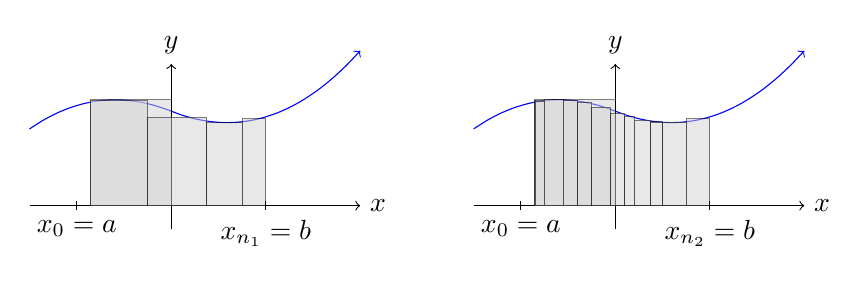
\begin{tikzpicture}[declare function = {f(\x) = 0.005 * \x^3 + 0.16 * \x^2 - 0.4 * \x + 2;}, scale = 0.6]

\def\offset{-4.7}

 \draw[->] ({-3 + \offset}, 0) -- ({4 + \offset}, 0) node[right] {$x$};
 \draw[->] ({0 + \offset}, -0.5) -- ({0 + \offset}, 3) node[above] {$y$};
  
  \draw[->, domain=-3:4, smooth, variable= \x, blue] plot ({\x + \offset}, {f(\x)});
  
  \def\lastx{-2}
  
	\foreach \x[count=\xi from 2, remember=\x as \lastx] in {-1.7, -0.5, 0.75, 1.5,  2} {
	\filldraw[color = black, fill = gray!35, opacity = 0.5] ({\lastx + \offset}, 0) -- ({\lastx +\offset}, {f(0.3 * \lastx + 0.7 * \x )}) -- ({\x + \offset}, {f(0.3 * \lastx + 0.7 * \x )}) -- ({\x + \offset}, 0) -- cycle;
}
      
  \draw ({-2 + \offset}, 0.1) -- ({-2 + \offset}, -0.1) node[below] {$x_0 = a$};
  \draw ({2 +\offset}, 0.1) -- ({2 + \offset}, -0.1) node[below] {$x_{n_1} = b$};  
  
\def\offset{4.7}

 \draw[->] ({-3 + \offset}, 0) -- ({4 + \offset}, 0) node[right] {$x$};
  \draw[->] ({0 + \offset}, -0.5) -- ({0 + \offset}, 3) node[above] {$y$};
  
  \draw[->, domain=-3:4, smooth, variable= \x, blue] plot ({\x + \offset}, {f(\x)});
  
  \def\lastx{-2}
  
	\foreach \x[count=\xi from 2, remember=\x as \lastx] in {-1.7, -1.5, -1.1, -0.8, -0.5, -0.1, 0.2, 0.4, 0.75, 1, 1.5,  2} {
	\filldraw[color = black, fill = gray!35, opacity = 0.5] ({\lastx + \offset}, 0) -- ({\lastx + \offset}, {f(0.3 * \lastx + 0.7 * \x )}) -- ({\x + \offset}, {f(0.3 * \lastx + 0.7 * \x )}) -- ({\x + \offset}, 0) -- cycle;
}
      
  \draw ({-2 + \offset}, 0.1) -- ({-2 + \offset}, -0.1) node[below] {$x_0 = a$};
  \draw ({2 +\offset}, 0.1) -- ({2 + \offset}, -0.1) node[below] {$x_{n_2} = b$};  
\end{tikzpicture}
\end{center}

The rectangles in the right figure do a better job of approximating the area under the curve. This is because the largest rectangle's width in the second figure is much smaller than the largest rectangle's width in the first.
\end{frame}

\begin{frame}
\frametitle{Partition Mesh}
\begin{Definition}
The {\bf mesh} of partition $P$ is
$$
\| P\| = \max\{\Delta x_1,\Delta x_2,\ldots \Delta x_n\}.
$$
\end{Definition}
As $\| P\|$ goes to 0, the approximation becomes better and better.
\end{frame}

\begin{frame}

%\begin{center}
%\begin{tikzpicture}[declare function = {f(\x) = 0.005 * \x^3 + 0.16 * \x^2 - 0.4 * \x + 2;}, scale = 0.7]

% \draw[->] (-3, 0) -- (4.2, 0) node[right] {$x$};
%  \draw[->] (0, -0.5) -- (0, 4.2) node[above] {$y$};
  
%  \draw[->, domain=-3:4.2, smooth, variable= \x, blue] plot ({\x}, {f(\x)}) node[right] {$y = f(x)$};
  
%  \def\lastx{-2}
  
%	\foreach \x[count=\xi from 2, remember=\x as \lastx] in {-1.7, -1.1, -0.5, 0.2, 0.75, 1, 1.5,  2}  {
%	\filldraw[color = black, fill = gray!35, opacity = 0.5] (\lastx, 0) -- (\lastx, {f(0.3 * \lastx + 0.7 * \x )}) -- (\x, {f(0.3 * \lastx + 0.7 * \x )}) -- (\x, 0) -- cycle;
%}
      
%  \draw (-2, 0.1) -- (-2, -0.1) node[below] {$x_0 = a$};
%  \draw (2, 0.1) -- (2, -0.1) node[below] {$x_n = b$};  
%\end{tikzpicture}
%\end{center}
\begin{Definition}
The {\bf Riemann integral} of $f$ over the interval $[a, b]$ is
$$
\int_a^b f(x)\ dx = \lim_{\|P\|\to 0} \sum_{k = 1}^n f(t_k) \Delta x_k
$$
whenever the limit converges. 
\end{Definition} 
\end{frame}

\begin{frame}
\frametitle{Integral Theorems}

\begin{Theorem}
A bounded function on an interval $[a, b]$ is Riemann integrable if it is continuous for all but a finite number of points. 
\end{Theorem}

\begin{Theorem}
If $f$ and $g$ are Riemann-integrable on $[a, b]$ and $\alpha$ and $\beta$ are constants, then the following hold.
\begin{enumerate}
\item[(a)] $\displaystyle \int_a^b \alpha f(x) + \beta g(x)\ dx = \alpha \int_a^b f(x)\ dx + \beta \int_a^b g(x)\ dx$
\item[(b)] $\displaystyle \int_a^b f(x)\ dx = \int_a^c f(x)\ dx + \int_c^b f(x)\ dx$ for any c in $[a, b]$
\end{enumerate}
\end{Theorem}
\end{frame}

\begin{frame}[t]
\frametitle{Analytic Example}
\small
\begin{Example}
Prove $\displaystyle\int_1^a \frac{dx}{x} = \ln a$ for $a > 1$. Use partition pairs of the form $P = (1, a^{1/n}, a^{2/n}\ldots, a)$ and $T = (1, a^{1/n}, a^{2/n}\ldots, a^{(n-1)/n})$.
\end{Example}
\end{frame}


\begin{frame}

\frametitle{Selection of $T$}
The most common choices for $T$ are
\begin{itemize}
\item Left endpoints:  $t_k = x_{k - 1}$
\item Right endpoints: $t_k = x_{k}$
\item Midpoints: $t_k = \frac{x_{k - 1} + x_{k}}{2}$
\end{itemize}

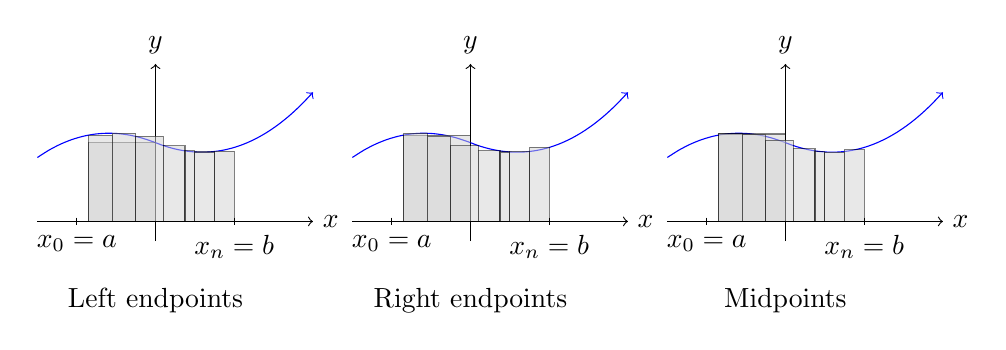
\begin{tikzpicture}[declare function = {f(\x) = 0.005 * \x^3 + 0.16 * \x^2 - 0.4 * \x + 2;}, scale = 0.5]

\def\offset{-8}

% Left endpoints
 \draw[->] ({-3 + \offset}, 0) -- ({4 + \offset}, 0) node[right] {$x$};
  \draw[->] (\offset, -0.5) -- (\offset, 4) node[above] {$y$};
  
  \draw[->, domain=-3:4, smooth, variable= \x, blue] plot ({\x + \offset}, {f(\x)});
  
  \def\lastx{-2}
  
	\foreach \x[count=\xi from 2, remember=\x as \lastx] in {-1.7, -1.1, -0.5, 0.2, 0.75, 1, 1.5,  2} {
	
	\filldraw[color = black, fill = gray!35, opacity = 0.5] ({\lastx + \offset}, 0) -- ({\lastx + \offset}, {f(\lastx)}) -- ({\x + \offset}, {f(\lastx)}) -- ({\x +\offset}, 0) -- cycle;
}
      
  \draw ({-2 + \offset}, 0.1) -- ({-2 + \offset}, -0.1) node[below] {$x_0 = a$};
  \draw ({2 + \offset}, 0.1) -- ({\offset + 2}, -0.1) node[below] {$x_n = b$};  
  
  \node at (\offset, -2) {Left endpoints};
  
  % Right endpoints
   \draw[->] (-3, 0) -- (4, 0) node[right] {$x$};
  \draw[->] (0, -0.5) -- (0, 4) node[above] {$y$};
  
  \draw[->, domain=-3:4, smooth, variable= \x, blue] plot ({\x}, {f(\x)});
  
  \def\lastx{-2}
  
	\foreach \x[count=\xi from 2, remember=\x as \lastx] in {-1.7, -1.1, -0.5, 0.2, 0.75, 1, 1.5,  2} {
	\filldraw[color = black, fill = gray!35, opacity = 0.5] (\lastx, 0) -- (\lastx, {f(\x)}) -- (\x, {f(\x)}) -- (\x, 0) -- cycle;
}
      
  \draw (-2, 0.1) -- (-2, -0.1) node[below] {$x_0 = a$};
  \draw (2, 0.1) -- (2, -0.1) node[below] {$x_n = b$};  
  
    \node at (0, -2) {Right endpoints};
    
  % Midpoints
  \def\offset{8}
  
  \draw[->] ({-3 + \offset}, 0) -- ({4 + \offset}, 0) node[right] {$x$};
  \draw[->] ({\offset}, -0.5) -- ({\offset}, 4) node[above] {$y$};
  
  \draw[->, domain=-3:4, smooth, variable= \x, blue] plot ({\x + \offset}, {f(\x)});
  
  \def\lastx{-2}
  
	\foreach \x[count=\xi from 2, remember=\x as \lastx] in {-1.7, -1.1, -0.5, 0.2, 0.75, 1, 1.5,  2} {
	\filldraw[color = black, fill = gray!35, opacity = 0.5] ({\lastx + \offset}, 0) -- ({\lastx + \offset}, {f(0.5 * \lastx + 0.5 * \x)}) -- ({\x + \offset}, {f(0.5 * \lastx + 0.5 * \x)}) -- ({\x +\offset}, 0) -- cycle;
}
      
  \draw ({-2 + \offset}, 0.1) -- ({-2 + \offset}, -0.1) node[below] {$x_0 = a$};
  \draw ({2 + \offset}, 0.1) -- ({2 + \offset}, -0.1) node[below] {$x_n = b$};  
  
      \node at (\offset, -2) {Midpoints};
 
\end{tikzpicture}

\end{frame}



\begin{frame}
\frametitle{Selection of $P$}
The most common choice for $P$, by far, is the uniform partition
$$
x_k = a + k \Delta x\qquad\text{and}\qquad \Delta x = \frac{b - a}{n}.
$$

\end{frame}

\begin{frame}
\frametitle{Useful formulas}
When working analytic problems with a uniform partition, these formulas come up a lot
$$
\sum_{k = 1}^n k = \frac{n(n + 1)}{2},\qquad \sum_{k = 1}^n k^2 = \frac{n(n+ 1)(2n+ 1)}{6}, 
$$
and
$$
\sum_{k = 1}^n k^3 = \frac{n^2(n+1)^2}{4} = \left[\frac{n(n+ 1)}{2}\right]^2.
$$
\end{frame}

\begin{frame}[t]
\frametitle{Uniform Partition Example}
\begin{Example}
Use uniform partitions and right endpoints to find $\displaystyle\int_0^1 x^2\ dx$.
\end{Example}
\end{frame}

\begin{frame}[fragile]
\frametitle{Python Code}
{
\linespread{0.8}
\tiny
\begin{verbatim*}
# Import numpy
import numpy as np

# Define Reimann sum
def riemann_sum(f, P, pts):
    
    # Sort values
    P = np.sort(P)

    # Calculate Delta x
    dxs = np.diff(P)

    # Calculate the number of terms
    N = len(dxs)
    
    # Define T
    if pts == 'left':

        T = [P[i] for i in range(0, N)]

    elif pts == 'right':

        T = [P[i + 1] for i in range(0, N)]

    elif pts == 'mid':
        
        T = [0.5 * P[i] + 0.5 * P[i + 1] for i in range(0, N)]
        
    # Get area of rectangles
    rectangles = [f(T[i]) * dxs[i] for i in range(0, N)]
    
    # Return sum
    return np.sum(rectangles) 
    \end{verbatim*}
 }
\end{frame}

\begin{frame}
\frametitle{Improper Integral}
\begin{Definition}
{
\linespread{0.5}
\begin{enumerate}
\item[(a)] If the integrals exists for every $t \geq a$ and for every $s \leq b$, then
$$
\int_a^\infty f(x)\ dx = \lim_{t\to\infty}\int_a^t f(x)\ dx\quad\text{and}\quad \int_{-\infty}^b f(x)\ dx = \lim_{s\to-\infty}\int_s^b f(x)\ dx.
$$
\item[(b)] For any $c$ in $\mathbb{R}$, if both $\displaystyle\int_c^\infty f(x)\ dx$ and $\displaystyle\int_{-\infty}^c f(x)\ dx$ converge, then 
$$
\int_{-\infty}^\infty f(x)\ dx = \int_{-\infty}^c f(x)\ dx + \int_c^\infty f(x)\ dx.
$$
\end{enumerate}
}
\end{Definition}
\end{frame}

\begin{frame}
\frametitle{Python Example}
\begin{Example}
Use \texttt{pandas} to create a data frame of Riemann sums with left endpoints, right endpoints, and midpoints, and uniform partitions to approximate $\displaystyle\int_0^\infty e^{-x^2/2}\ dx$. Consider $n = 10, 50, 100, 500,$ and 1000.
\end{Example}
\end{frame}

\begin{frame}[fragile]
\frametitle{Python Example Cont.}

{\bf Solution. } Since $e^{-x^2/2}$ goes to 0 rapidly, it's safe to use $b = 10$. 
{
\linespread{0.8}
\tiny
\begin{verbatim*}
# Import pandas
import pandas as pd

# Define function
f = lambda x: np.e**(-x**2/2)

# Define the n-values
n_vals = [10, 50, 100, 500, 1000]

# Define the data frame
results = pd.DataFrame(index = n_vals, columns = ['left', 'right', 'mid'])

# Loop over values
for n in n_vals:
    
    # We can use np.linspace for a uniform partition
    partition = np.linspace(0, 10, n + 1)
    
    # Get left endpoint results
    results.loc[n, 'left'] = riemann_sum(f, partition, 'left')
 
    # Get right endpoint results
    results.loc[n, 'right'] = riemann_sum(f, partition, 'right')
    
    # Get midpoint results
    results.loc[n, 'mid'] = riemann_sum(f, partition, 'mid')    
\end{verbatim*}
}
\end{frame}

\begin{frame}[fragile]
\frametitle{Python Example Result}
The limit as the mesh of $P$ goes to 0 is $\sqrt{\pi/2}\approx 1.253$.
\begin{center}
\includegraphics[scale = 0.8]{ex4.png}
\end{center}
\end{frame}

\subsection{Indefinite Integration} 


\begin{frame}
\frametitle{Indefinite Integral}

\begin{Definition}
The function $F$ is an {\bf indefinite integral} or {\bf antiderivative} of $f$ if $F\ '(x) = f(x)$. We write
$$
\int f(x)\ dx = F(x)
$$
to denote this.
\end{Definition}
Indefinite integrals are only unique up to a constant. For example, two antiderivatives of $2x$ are $x^2 +1$ and $x^2 - 4$. To handle all possibilities, we write
$$
\int 2x\ dx = x^2 + C.
$$
\end{frame}


\begin{frame}
\frametitle{Antiderivative Theorems}
\begin{Theorem}
Let $f$ and $g$ be continuous functions on some domain and let $\alpha$ and $\beta$ be real numbers. Then
$$
\int \alpha f(x) + \beta g(x)\ dx = \alpha \int f(x)\ dx + \beta \int g(x)\ dx.
$$
\end{Theorem}
\end{frame}

\begin{frame}
\frametitle{Useful Antiderivative Formulas}
\begin{multicols}{2}
{\small 
\begin{itemize}
\item $\displaystyle \int x^n\ dx = \frac{1}{n+ 1} x^{n+ 1} + C$, $n\neq -1$
\item $\displaystyle \int \frac{dx}{x} = \ln|x| + C$	
\item $\displaystyle \int \frac{dx}{1 + x^2} = \arctan x + C$	
\item $\displaystyle \int e^x\ dx  = e^x + C$
\item $\displaystyle \int a^x\ dx = \frac{a^x}{\ln x} + C$
\item $\displaystyle\int \sin x\ dx = -\cos x + C$
\item $\displaystyle \int cos x\ dx= \sin x + C$
\item $\displaystyle\int \tan x\ dx = -\ln|cos x| + C$
\end{itemize}
}
\end{multicols}

\end{frame}

\begin{frame}
\frametitle{Fundamental Theorem of Calculus}

\begin{Theorem}[Fundamental Theorem of Calculus]
Suppose $f$ is continuous on the closed interval $[a, b]$. Then
\begin{enumerate}
\item[(a)] $\displaystyle\int_a^b f(x)\ dx = F(b) - F(a)$, where $F\ '(x)= f(x)$.
\item[(b)] $\displaystyle\frac{d}{dx}\left(\int_a^x f(t)\ tx\right) = f(x)$
\end{enumerate}
\end{Theorem}
\end{frame}

\begin{frame}[t]
\frametitle{Example}

\begin{Example}
$\displaystyle \int_0^2 \max\{x, 1\}\ dx = $
\end{Example}

\end{frame}

\begin{frame}
\frametitle{Proof of the Fundamental Theorem on YouTube}
Watch Peyam prove part (b) of the Fundamental Theorem of Calculus  (\url{https://youtu.be/4DrCKhCECHo}).
\begin{center}
\includegraphics[scale = 0.25]{peyam.png}
\end{center}
\end{frame}

\begin{frame}
\frametitle{u-Substitution} 

\begin{Theorem}[u-Substitution]
Suppose $g\ '$ is continuous on the closed interval $[a, b]$ and $f$ is continuous on the range of $g$. Then
$$
\int_a^b (f \circ g)(x)\cdot g\ '(x)\ dx = \int_{g(a)}^{g(b)} f(u)\ du.
$$
\end{Theorem}
\end{frame}

\begin{frame}[t]
\frametitle{Example}
\begin{Example}
$\displaystyle \int x e^{-x^2/2}\ dx =$
\end{Example}

\end{frame}

\begin{frame}
\frametitle{Integration by Parts}

\begin{Theorem}[Integration by parts]
Suppose $F$ and $G$ are differentiable functions, $F\ '(x) = f(x)$, and $G\ '(x) = g(x)$, where $f$ and $g$ are continuous. Then
$$
\int F(x) g(x)\ dx = F(x) G(x) - \int f(x) G(x)\ dx.
$$
\end{Theorem}
\end{frame}

\begin{frame}[t]
\frametitle{Example}
\begin{Example}
$\displaystyle\int \ln x\ dx = $
\end{Example}
\end{frame}

\section{Ordinary Differential Equations}

\begin{frame}
\frametitle{Ordinary Differential Equations}

\begin{Definition}
\begin{enumerate}
\item[(a)] An {\bf ordinary differential equation} (ODE) involves an unknown function of a single variable and some of its derivatives. 
\item[(b)] The {\bf order} of a differential equation is the order of the highest derivative that appears in the equation.
\end{enumerate}
\end{Definition} 
For example, $x y\; ' = e^{xy}$ is a first order ordinary differential equation, while
$$
\frac{d^3 x}{dt^3} - 2t\dfrac{d^2x}{dt^2} + t^2 x = \cos t
$$
is a third order ordinary differential equation.

\end{frame}

\subsection{Separable ODEs}

\begin{frame}
\frametitle{Separable ODEs}
\begin{Definition}
An ODE of the form
$$
\frac{dy}{dx} = F(x, y)
$$
is separable if $F(x, y) = f(x) g(y)$.
\end{Definition}
It's relatively easy to solve separable differential equations 
$$
\frac{dy}{dx} =  f(x) g(y)\qquad\text{implies}\qquad \frac{1}{g(y)} \frac{dy}{dx}  = f(x).
$$
Hence,
$$
\int \frac{1}{g(y)} \frac{dy}{dx}\ dx = \int f(x)\ dx\qquad\text{implies}\qquad \int \frac{1}{g(y)}\ dy = \int f(x)\ dx.
$$
\end{frame}

\begin{frame}[t]
\frametitle{Separable ODE Example}
\small
\begin{Example}
Solve the differential equation
$$
\frac{dy}{dt} = \frac{ty + 3t}{t^2 + 1}
$$
subject to the initial condition $y(2) = 2$.
\end{Example}
\end{frame}

\subsection{First Order Linear ODEs}
\begin{frame}
\frametitle{Linear ODEs}
\begin{Definition}
A first order {\bf linear} differential equation is one that can be written in the form
$$
\frac{dy}{dx} + P(x) y = Q(x).
$$
\end{Definition}
The idea behind solving these is to find $\mu = f(x)$ such that
$$
\frac{d}{dx}\left(\mu y\right) = \mu \frac{dy}{dx} + \mu P(x) y.
$$
Using the product rule, it becomes clear
$$
\frac{d\mu}{dx} = \mu P(x)\qquad\text{implies}\qquad \mu = \exp\left(\int P(x)\ dx\right).
$$
\end{frame}

\begin{frame}[t]
\frametitle{Linear ODEs Example}
\small
\begin{Example}
Solve the differential equation 
$$
x\frac{dy}{dx} + 3x^3y = 6 x^3.
$$
\end{Example}
\end{frame}

\end{document}
